\documentclass{standalone}
\usepackage{tikz}
\usetikzlibrary{patterns, positioning}

\begin{document}
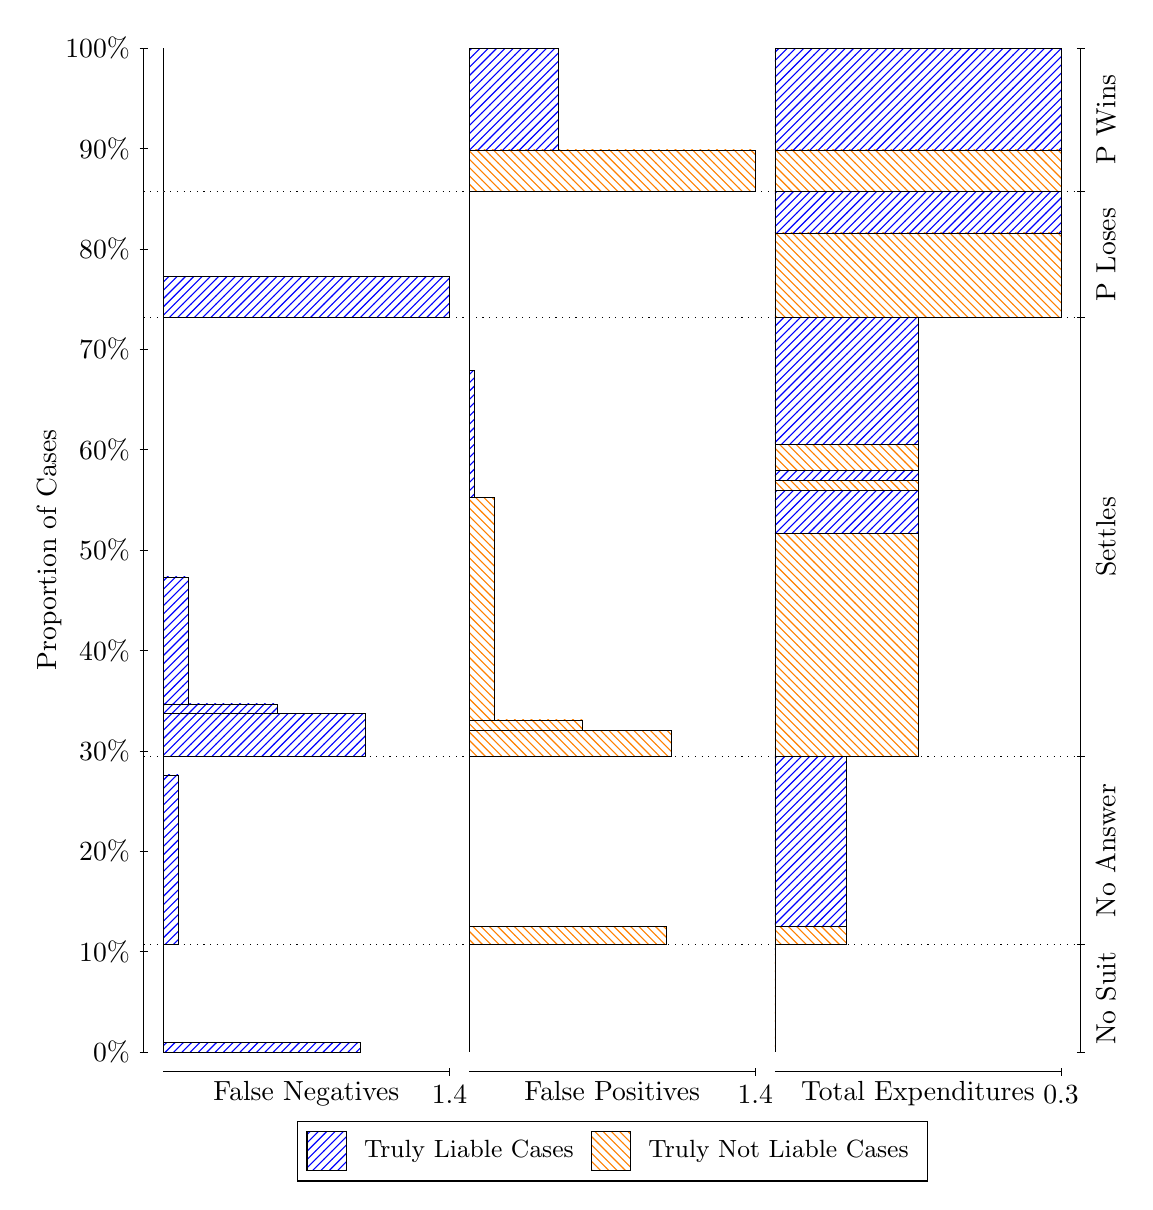
\begin{tikzpicture}
\draw[black, very thin] (1.5,1.75) -- (1.5,14.5);
\node[rotate=90, anchor=center] at (0.3, 8.125) {Proportion of Cases};
\draw[black, very thin] (1.45,1.75) -- (1.55,1.75);
\node[anchor=east] at (1.45, 1.75) {0\%};
\draw[black, very thin] (1.45,3.025) -- (1.55,3.025);
\node[anchor=east] at (1.45, 3.025) {10\%};
\draw[black, very thin] (1.45,4.3) -- (1.55,4.3);
\node[anchor=east] at (1.45, 4.3) {20\%};
\draw[black, very thin] (1.45,5.575) -- (1.55,5.575);
\node[anchor=east] at (1.45, 5.575) {30\%};
\draw[black, very thin] (1.45,6.85) -- (1.55,6.85);
\node[anchor=east] at (1.45, 6.85) {40\%};
\draw[black, very thin] (1.45,8.125) -- (1.55,8.125);
\node[anchor=east] at (1.45, 8.125) {50\%};
\draw[black, very thin] (1.45,9.4) -- (1.55,9.4);
\node[anchor=east] at (1.45, 9.4) {60\%};
\draw[black, very thin] (1.45,10.675) -- (1.55,10.675);
\node[anchor=east] at (1.45, 10.675) {70\%};
\draw[black, very thin] (1.45,11.95) -- (1.55,11.95);
\node[anchor=east] at (1.45, 11.95) {80\%};
\draw[black, very thin] (1.45,13.225) -- (1.55,13.225);
\node[anchor=east] at (1.45, 13.225) {90\%};
\draw[black, very thin] (1.45,14.5) -- (1.55,14.5);
\node[anchor=east] at (1.45, 14.5) {100\%};

\draw[black, very thin] (13.4,1.75) -- (13.4,14.5);
\draw[black, very thin] (13.35,1.75) -- (13.45,1.75);
\node[anchor=west] at (13.35, 1.75) {};
\draw[black, very thin] (13.35,3.112) -- (13.45,3.112);
\node[anchor=west] at (13.35, 3.112) {};
\draw[black, very thin] (13.35,5.5053) -- (13.45,5.5053);
\node[anchor=west] at (13.35, 5.5053) {};
\draw[black, very thin] (13.35,11.077) -- (13.45,11.077);
\node[anchor=west] at (13.35, 11.077) {};
\draw[black, very thin] (13.35,12.68) -- (13.45,12.68);
\node[anchor=west] at (13.35, 12.68) {};
\draw[black, very thin] (13.35,14.5) -- (13.45,14.5);
\node[anchor=west] at (13.35, 14.5) {};

\draw[black, very thin, pattern color=blue, pattern=north east lines] (1.75,1.75) rectangle (4.2557,1.8697);
\draw[black, very thin, pattern color=orange, pattern=north west lines] (1.75,1.8697) rectangle (1.75,3.112);
\draw[black, very thin, pattern color=blue, pattern=north east lines] (1.75,3.112) rectangle (1.9379,5.2682);
\draw[black, very thin, pattern color=orange, pattern=north west lines] (1.75,5.2682) rectangle (1.75,5.5053);
\draw[black, very thin, pattern color=blue, pattern=north east lines] (1.75,5.5053) rectangle (4.3184,6.0493);
\draw[black, very thin, pattern color=blue, pattern=north east lines] (1.75,6.0493) rectangle (3.1908,6.1719);
\draw[black, very thin, pattern color=blue, pattern=north east lines] (1.75,6.1719) rectangle (2.0632,7.7842);
\draw[black, very thin, pattern color=orange, pattern=north west lines] (1.75,7.7842) rectangle (1.75,11.077);
\draw[black, very thin, pattern color=blue, pattern=north east lines] (1.75,11.077) rectangle (5.3833,11.604);
\draw[black, very thin, pattern color=orange, pattern=north west lines] (1.75,11.604) rectangle (1.75,12.68);
\draw[black, very thin, pattern color=orange, pattern=north west lines] (1.75,12.68) rectangle (1.75,13.207);
\draw[black, very thin, pattern color=blue, pattern=north east lines] (1.75,13.207) rectangle (1.75,14.5);
\draw[black, very thin, pattern color=orange, pattern=north west lines] (5.6333,1.75) rectangle (5.6333,2.9923);
\draw[black, very thin, pattern color=blue, pattern=north east lines] (5.6333,2.9923) rectangle (5.6333,3.112);
\draw[black, very thin, pattern color=orange, pattern=north west lines] (5.6333,3.112) rectangle (8.1391,3.3491);
\draw[black, very thin, pattern color=blue, pattern=north east lines] (5.6333,3.3491) rectangle (5.6333,5.5053);
\draw[black, very thin, pattern color=orange, pattern=north west lines] (5.6333,5.5053) rectangle (8.2017,5.8382);
\draw[black, very thin, pattern color=orange, pattern=north west lines] (5.6333,5.8382) rectangle (7.0741,5.9675);
\draw[black, very thin, pattern color=orange, pattern=north west lines] (5.6333,5.9675) rectangle (5.9466,8.7978);
\draw[black, very thin, pattern color=blue, pattern=north east lines] (5.6333,8.7978) rectangle (5.696,10.41);
\draw[black, very thin, pattern color=blue, pattern=north east lines] (5.6333,10.41) rectangle (5.6333,11.077);
\draw[black, very thin, pattern color=orange, pattern=north west lines] (5.6333,11.077) rectangle (5.6333,12.153);
\draw[black, very thin, pattern color=blue, pattern=north east lines] (5.6333,12.153) rectangle (5.6333,12.68);
\draw[black, very thin, pattern color=orange, pattern=north west lines] (5.6333,12.68) rectangle (9.2667,13.207);
\draw[black, very thin, pattern color=blue, pattern=north east lines] (5.6333,13.207) rectangle (6.7609,14.5);
\draw[black, very thin, pattern color=orange, pattern=north west lines] (9.5167,1.75) rectangle (9.5167,2.9923);
\draw[black, very thin, pattern color=blue, pattern=north east lines] (9.5167,2.9923) rectangle (9.5167,3.112);
\draw[black, very thin, pattern color=orange, pattern=north west lines] (9.5167,3.112) rectangle (10.425,3.3491);
\draw[black, very thin, pattern color=blue, pattern=north east lines] (9.5167,3.3491) rectangle (10.425,5.5053);
\draw[black, very thin, pattern color=orange, pattern=north west lines] (9.5167,5.5053) rectangle (11.333,8.3356);
\draw[black, very thin, pattern color=blue, pattern=north east lines] (9.5167,8.3356) rectangle (11.333,8.8796);
\draw[black, very thin, pattern color=orange, pattern=north west lines] (9.5167,8.8796) rectangle (11.333,9.0088);
\draw[black, very thin, pattern color=blue, pattern=north east lines] (9.5167,9.0088) rectangle (11.333,9.1314);
\draw[black, very thin, pattern color=orange, pattern=north west lines] (9.5167,9.1314) rectangle (11.333,9.4644);
\draw[black, very thin, pattern color=blue, pattern=north east lines] (9.5167,9.4644) rectangle (11.333,11.077);
\draw[black, very thin, pattern color=orange, pattern=north west lines] (9.5167,11.077) rectangle (13.15,12.153);
\draw[black, very thin, pattern color=blue, pattern=north east lines] (9.5167,12.153) rectangle (13.15,12.68);
\draw[black, very thin, pattern color=orange, pattern=north west lines] (9.5167,12.68) rectangle (13.15,13.207);
\draw[black, very thin, pattern color=blue, pattern=north east lines] (9.5167,13.207) rectangle (13.15,14.5);
\draw[black, dotted] (1.5,3.112) -- (13.4,3.112);
\draw[black, dotted] (1.5,5.5053) -- (13.4,5.5053);
\draw[black, dotted] (1.5,11.077) -- (13.4,11.077);
\draw[black, dotted] (1.5,12.68) -- (13.4,12.68);
\draw[black, very thin] (1.75,1.5) -- (5.3833,1.5);
\node[anchor=north] at (3.5667, 1.5) {False Negatives};
\draw[black, very thin] (5.3833,1.45) -- (5.3833,1.55);
\node[anchor=north] at (5.3833, 1.45) {1.4};

\draw[black, very thin] (5.6333,1.5) -- (9.2667,1.5);
\node[anchor=north] at (7.45, 1.5) {False Positives};
\draw[black, very thin] (9.2667,1.45) -- (9.2667,1.55);
\node[anchor=north] at (9.2667, 1.45) {1.4};

\draw[black, very thin] (9.5167,1.5) -- (13.15,1.5);
\node[anchor=north] at (11.333, 1.5) {Total Expenditures};
\draw[black, very thin] (13.15,1.45) -- (13.15,1.55);
\node[anchor=north] at (13.15, 1.45) {0.3};

\node[black, centered, rotate=90] at (13.72, 2.431) {No Suit};
\node[black, centered, rotate=90] at (13.72, 4.3086) {No Answer};
\node[black, centered, rotate=90] at (13.72, 8.291) {Settles};
\node[black, centered, rotate=90] at (13.72, 11.878) {P Loses};
\node[black, centered, rotate=90] at (13.72, 13.59) {P Wins};

\draw (7.449999999999999,1.5) node[draw=none] (baseCoordinate) {};
\begin{scope}[align=center]
        \matrix[scale=0.5, draw=black, below=0.5cm of baseCoordinate, nodes={draw}, column sep=0.1cm]{
            \node[rectangle, draw, minimum width=0.5cm, minimum height=0.5cm, pattern=north east lines, pattern color=blue] {}; &
            \node[draw=none, font=\small] (B) {Truly Liable Cases}; &
            \node[rectangle, draw, minimum width=0.5cm, minimum height=0.5cm, pattern=north west lines, pattern color=orange] {}; &
            \node[draw=none, font=\small] (B) {Truly Not Liable Cases}; \\
            };
\end{scope}

\end{tikzpicture}
\end{document}